% !TEX root = ../main.tex
%----------------------------------------------------------------------------------------

\chapter{Example Walkthrough} 
\label{ChapterExampleWalkthrough}

%----------------------------------------------------------------------------------------

The previous chapter described the CorpusAgent system from an architectural and methodological perspective, detailing the individual pipeline layers and their interactions. While this abstraction is necessary to understand the design rationale and technical capabilities of the system, it does not directly indicate how these components manifest in an actual system execution.

This chapter therefore provides an example walkthrough of the CorpusAgent interface from a system-level UI perspective. The walkthrough illustrates how the previously introduced architectural components are reflected in the interface and how they interact during a concrete pipeline run. \\
For each stage, the corresponding UI elements are presented alongside brief references to the underlying technical processes described in Chapter~\ref{ChapterMethodology}

\section{Step 1 - Entering a Question}

\begin{figure}[ht]
    \centering
    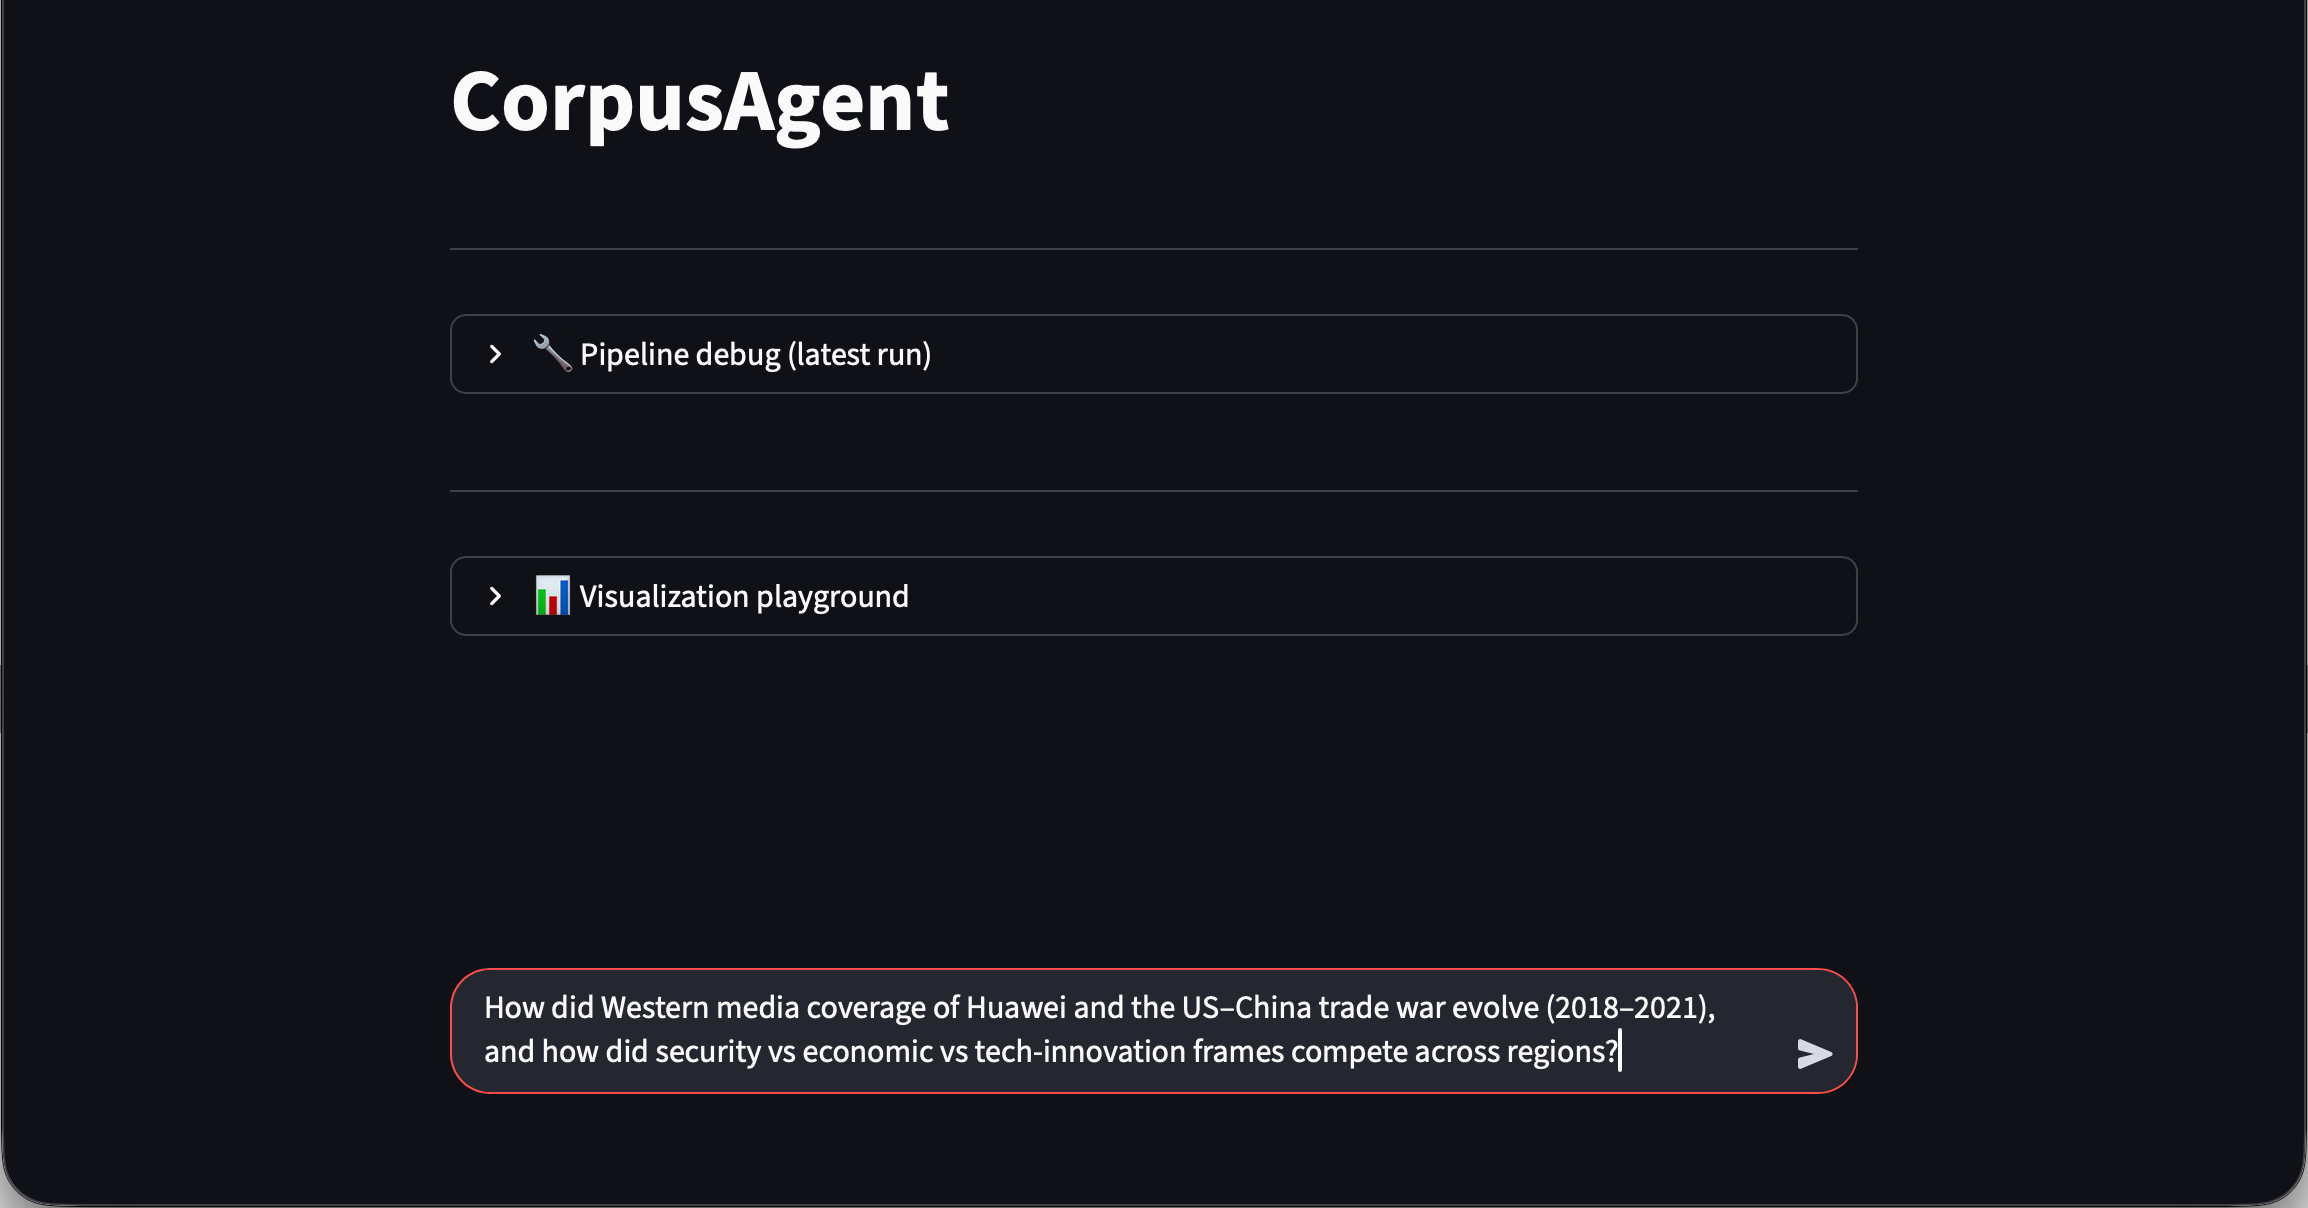
\includegraphics[width=0.95\textwidth]{Figures/walkthrough/ui_01_query_entry.png}
    \caption{CorpusAgent landing view with collapsible panels and query input field.}
    \label{fig:ui-query-entry}
\end{figure}

The application starts in a minimal state, exposing two collapsible system panels ("Pipeline debug" and "Visualization playground") and a persistent query input field (Figure~\ref{fig:ui-query-entry}). Submitting a query triggers the pipeline run, which then persists run metadata and intermediate artifacts for later inspection.

\section{Step 2 - Pipeline execution State}

\begin{figure}[ht]
    \centering
    
\includegraphics[width=0.95\textwidth]{Figures/walkthrough/ui_02_running_state.png}
    \caption{Query submitted; the system indicates an active run (retrieval + NLP execution).}
    \label{fig:ui-running}
\end{figure}

After submission, the UI transitions into a run state and displays an execution indicator (Figure~\ref{fig:ui-running}). Internally, this corresponds to the orchestration of retrieval and subsequent processing stages, as described in the section Pipeline orchestration \ref{PipelinePlanningLayer}.

\section{Step 3 - Final synthesized answer}

\begin{figure}[ht]
    \centering
    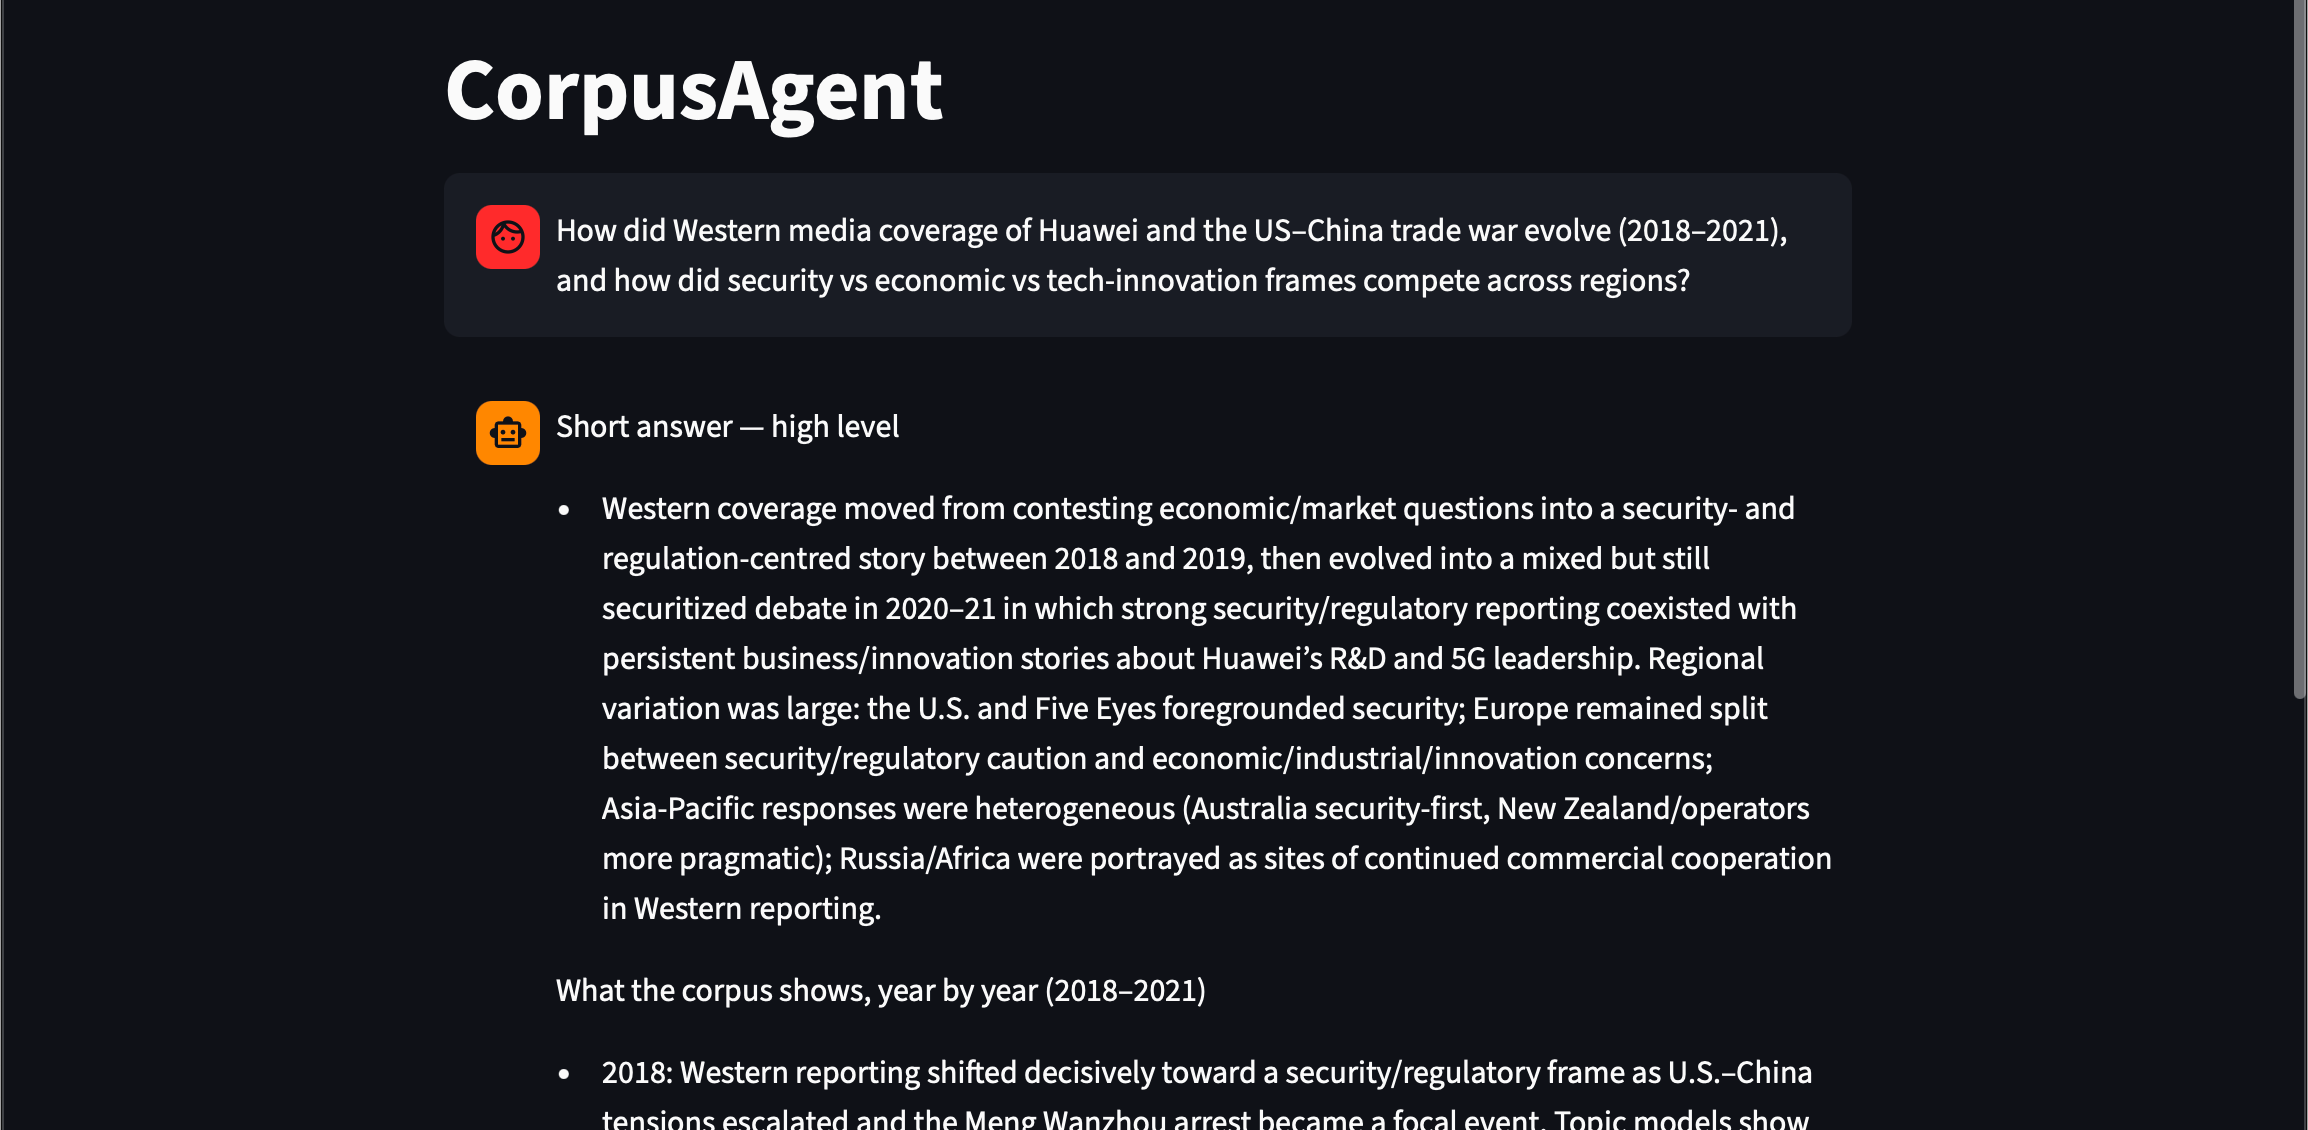
\includegraphics[width=0.95\textwidth]{Figures/walkthrough/ui_03_final_answer.png}
    \caption{Final synthesized answer displayed in the UI after pipeline completion.}
    \label{fig:ui-final-answer}
\end{figure}

Once the run completes, the final LLM-synthesized response is rendered in the chat view (Figure~\ref{fig:ui-final-answer}). This output corresponds to the terminal synthesis stage, where temporally aggregated evidence is transformed into a structured narrative answer.

\FloatBarrier

\section{Step 4 - Run introspection via "Pipeline debug"}

\begin{figure}[H]
    \centering
    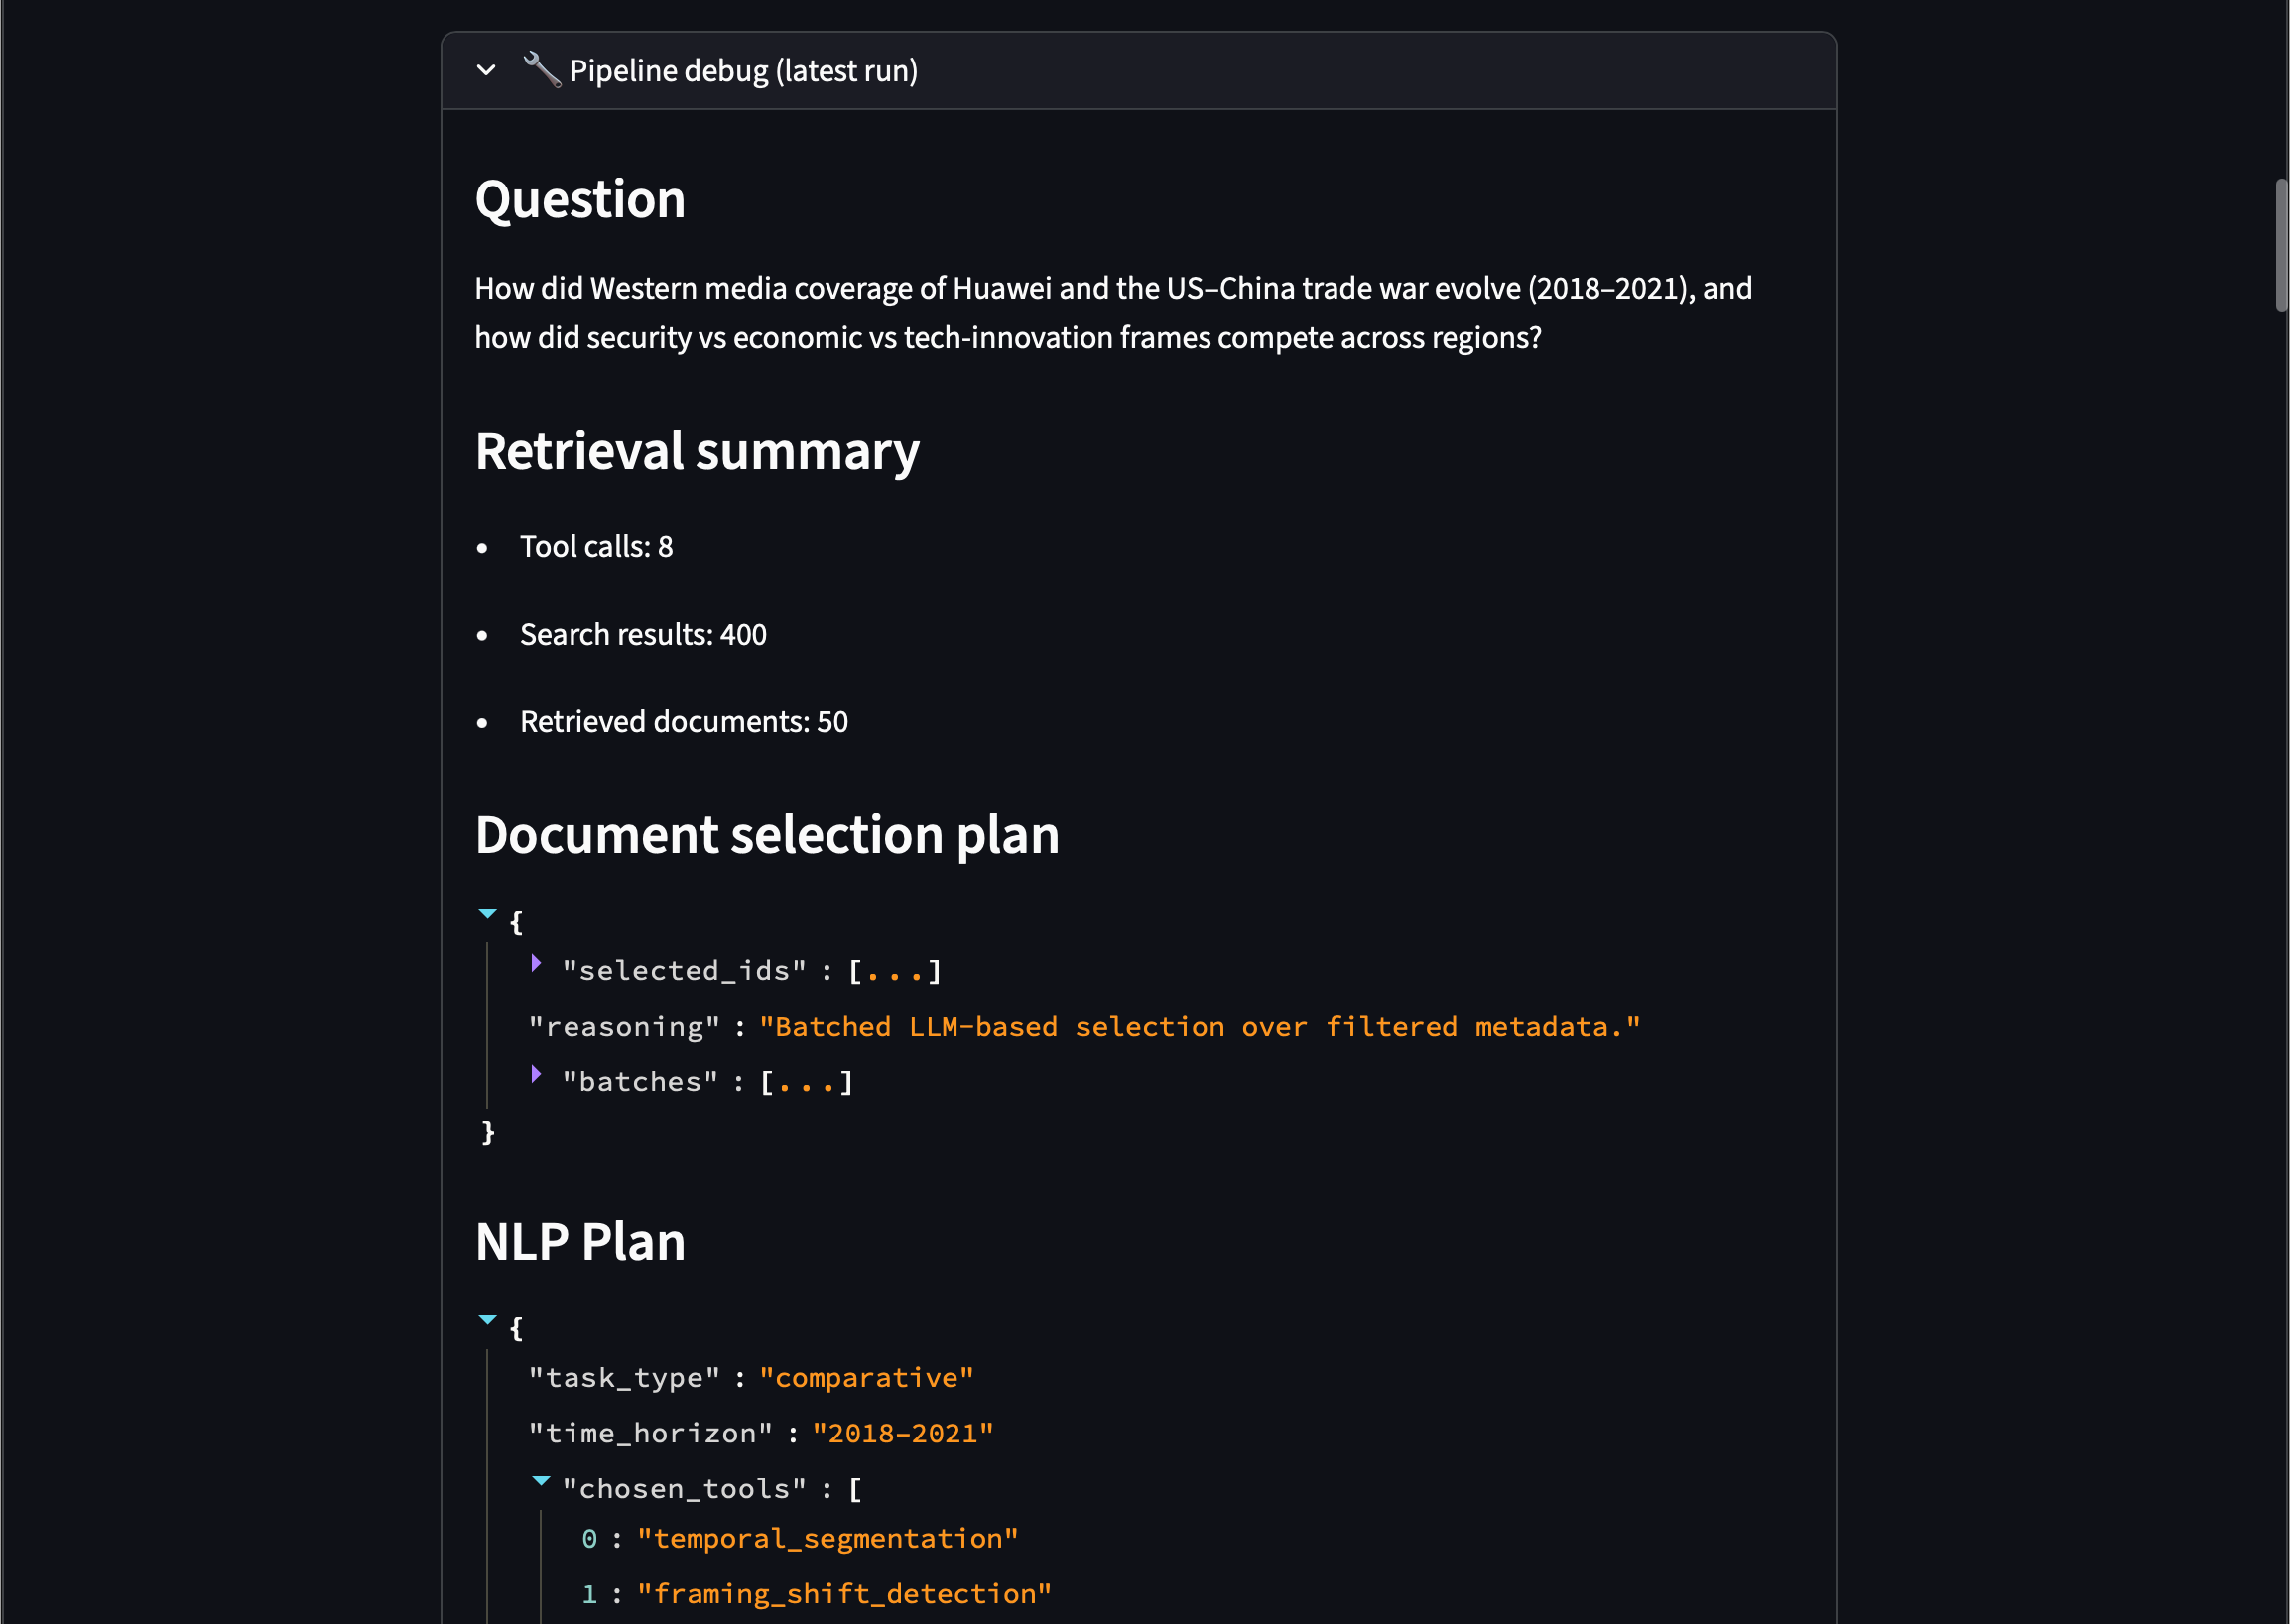
\includegraphics[width=0.95\textwidth]{Figures/walkthrough/ui_04_pipeline_debug.png}
    \caption{Expanded "Pipeline debug" panel showing detailed run metadata and intermediate artifacts.}
    \label{fig:ui-pipeline-debug}
\end{figure}

For transparency and debugging, the "Pipeline debug" panel exposes structured artifacts from the latest run (Figure~\ref{fig:ui-pipeline-debug}). This includes a compact retrieval summary (e.g., number of tool calls and retrieved documents), as well as JSON-based planning outputs such as the document selection plan and the NLP plan. These artifacts allow the run’s internal decision-making to be inspected independently of the final answer.

\FloatBarrier

\section{Step 5 - Accessing the Visualization Playground}

\begin{figure}[H]
    \centering
    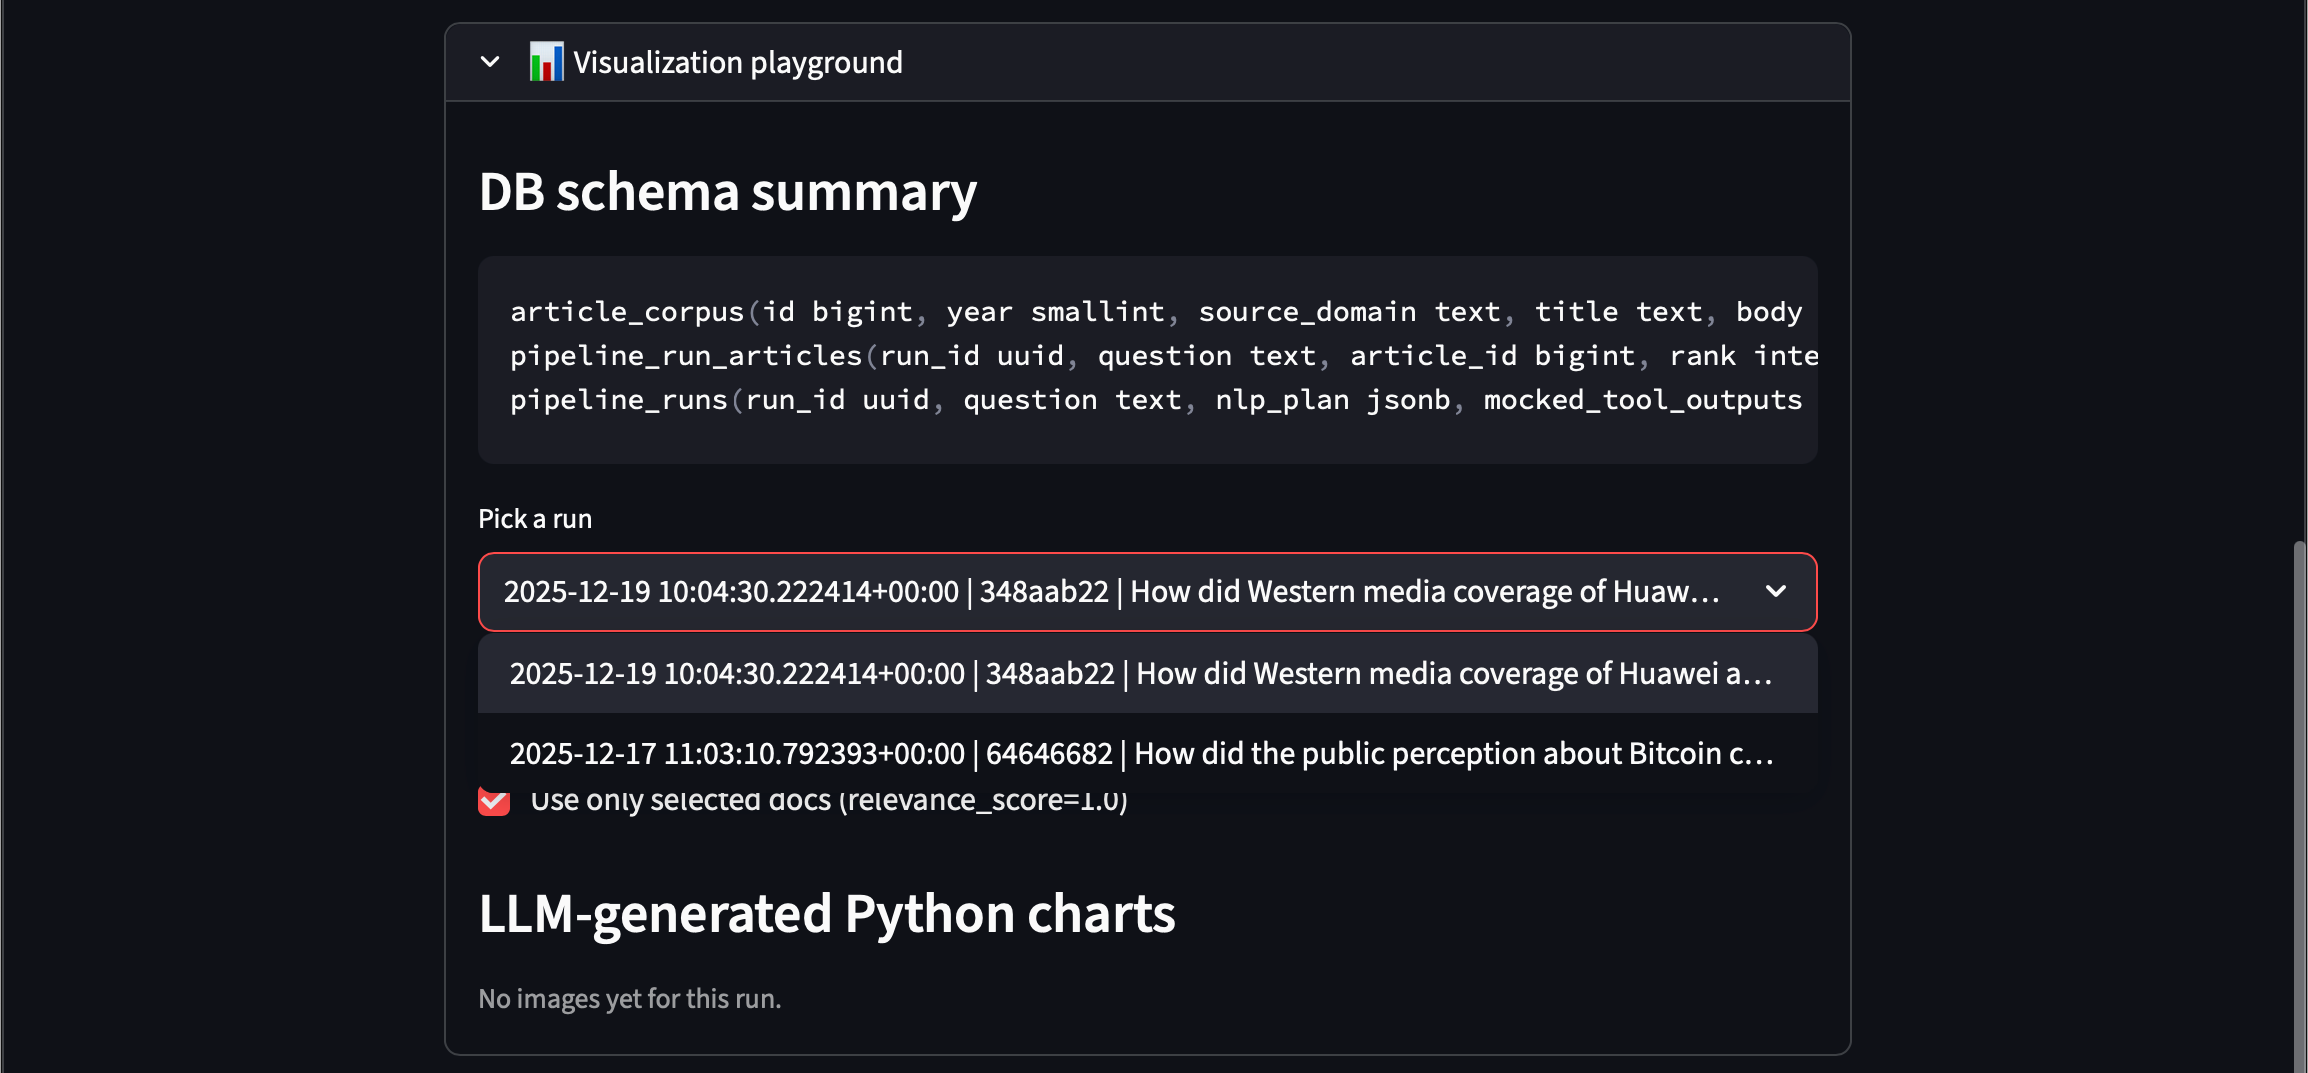
\includegraphics[width=0.95\textwidth]{Figures/walkthrough/ui_05_viz_playground_overview.png}
    \caption{Visualization Playground panel with schema summary and run selection.}
    \label{fig:ui-viz-playground}
\end{figure}

The "Visualization playground" is exposed as a separate panel that operates on stored run data (Figure~\ref{fig:ui-viz-playground}). The UI displays a condensed database schema summary and provides a dropdown to select a run. This design makes the visualization generation reproducible and run-centric: all charts are explicitly tied to a run\_id.

\FloatBarrier

\section{Step 6 - LLM-generated visualization plan (JSON)}

\begin{figure}[H]
    \centering
    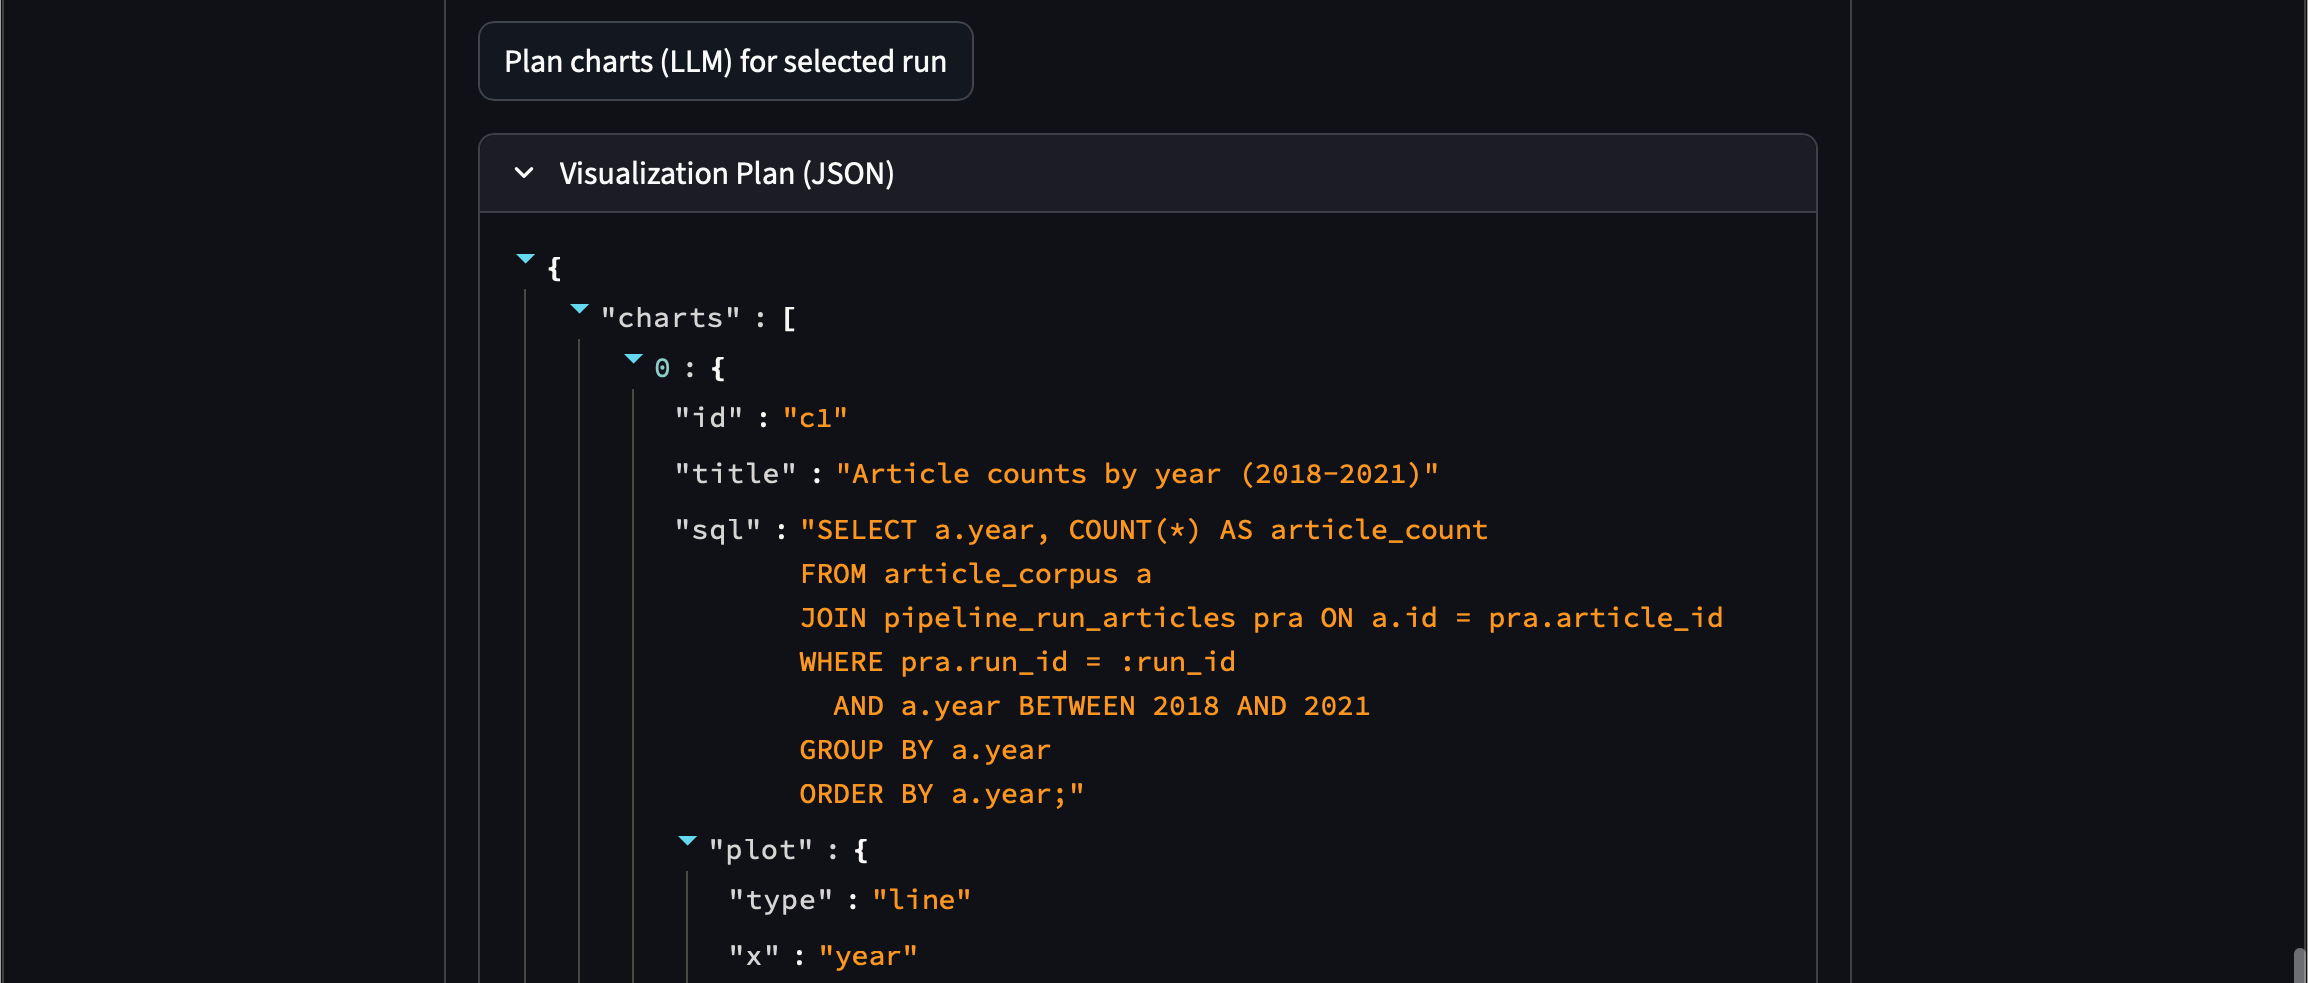
\includegraphics[width=0.95\textwidth]{Figures/walkthrough/ui_06_viz_plan_json.png}
    \caption{Visualization Plan in JSON form, including SQL queries and plot specifications.}
    \label{fig:ui-viz-plan}
\end{figure}

After selecting a run, the system generates a visualization plan (Figure~\ref{fig:ui-viz-plan}). The plan is represented as structured JSON containing (i) chart identifiers and titles, (ii) SQL queries scoped to the selected run\_id, and (iii) lightweight plot specifications (e.g., plot type and axis bindings). This plan serves as an intermediate, inspectable representation before any code is executed.

\FloatBarrier

\section{Step 7 - Generated plotting code (Python)}

\begin{figure}[H]
    \centering
    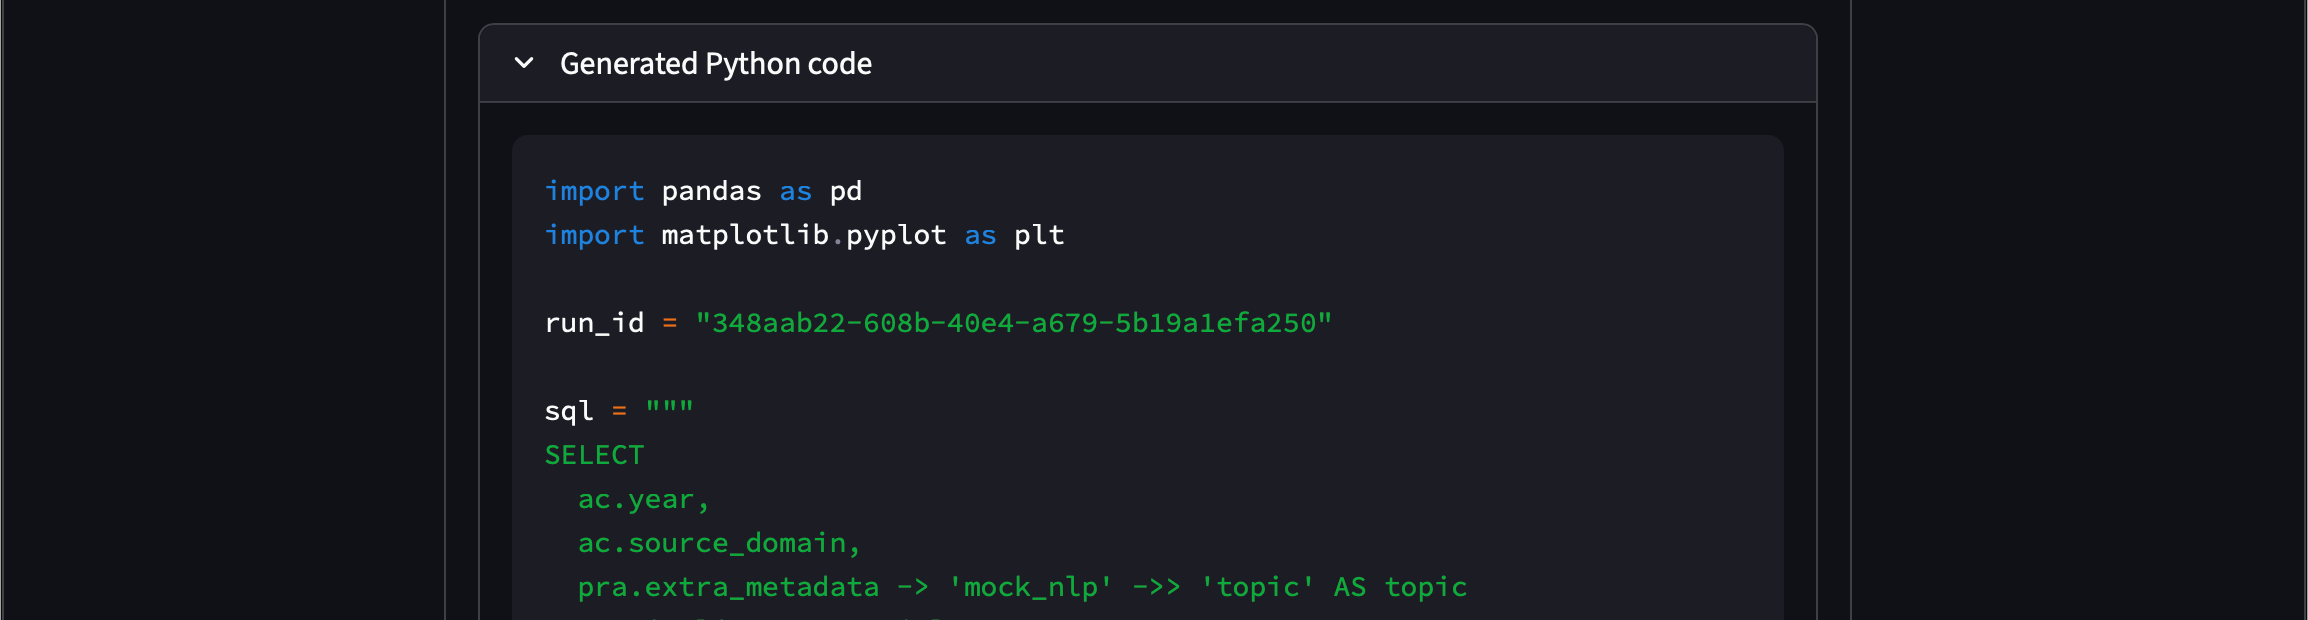
\includegraphics[width=0.95\textwidth]{Figures/walkthrough/ui_07_generated_code.png}
    \caption{LLM-generated Python code used to query the database and render charts.}
    \label{fig:ui-generated-code}
\end{figure}

Based on the JSON plan, the system generates executable Python code (Figure~\ref{fig:ui-generated-code}). The code queries the working dataset for the selected run, performs minimal transformations (e.g., normalizing labels into a small set of frames), and renders charts with Matplotlib. Persisting this code can be used for reproducibility and for diagnosing failures when chart generation does not succeed.

\FloatBarrier

\section{Step 8 - Chart rendering and output inspection}

\begin{figure}[H]
    \centering
    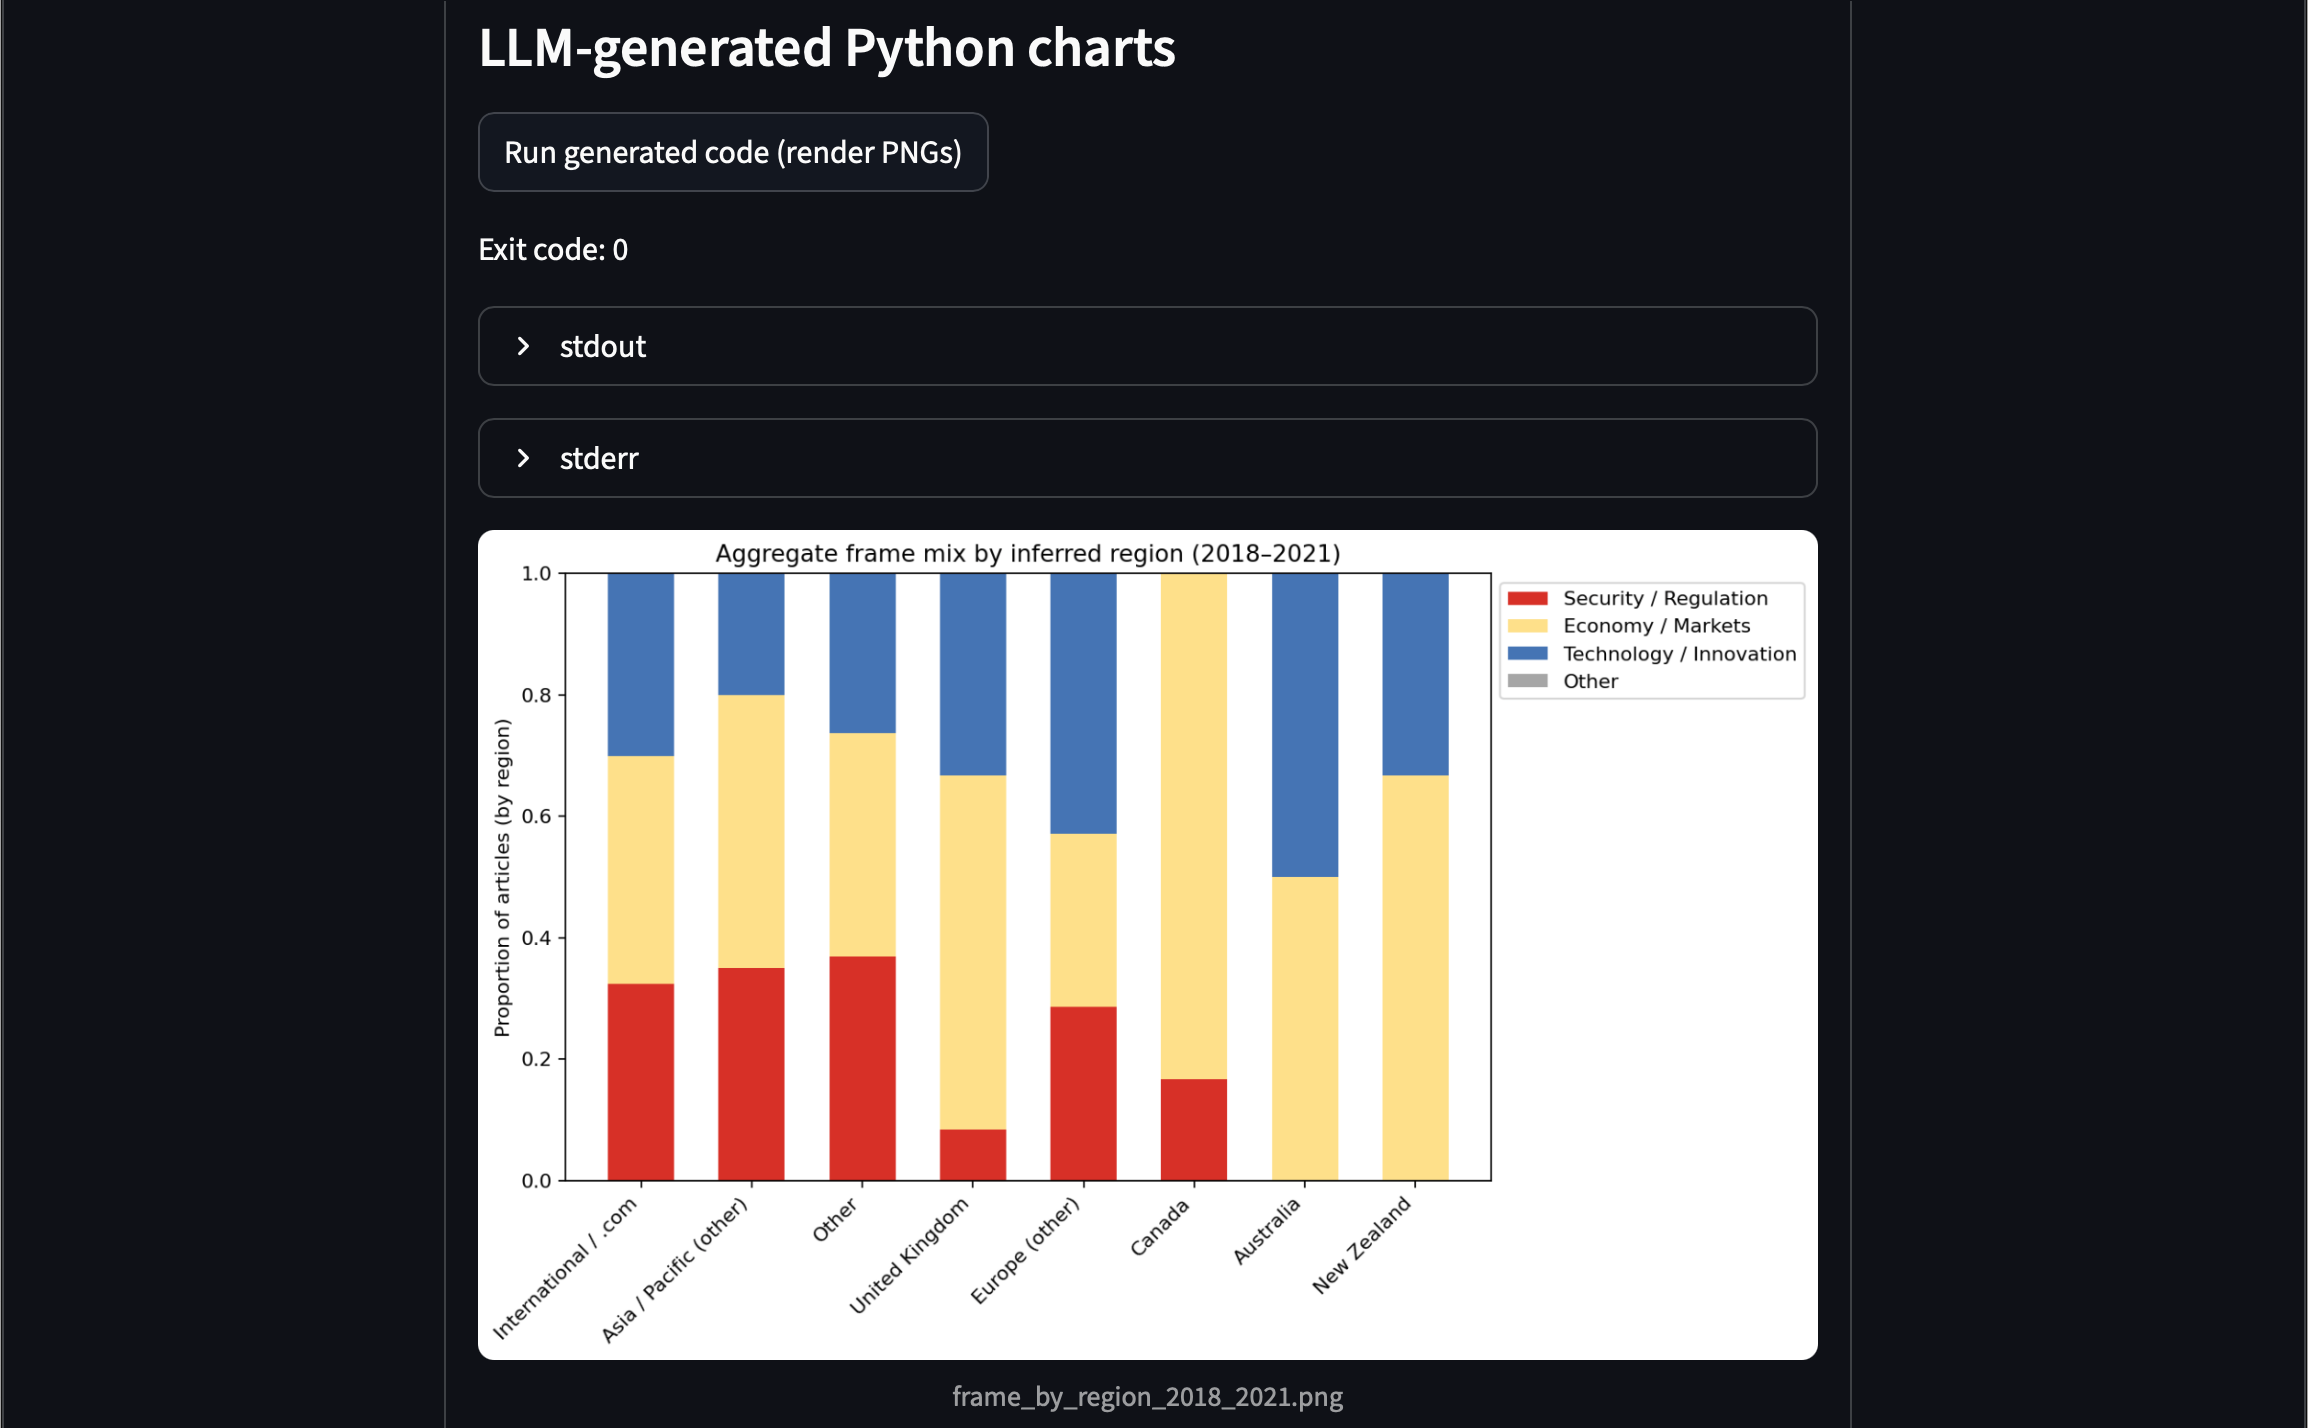
\includegraphics[width=0.95\textwidth]{Figures/walkthrough/ui_08_rendered_charts.png}
    \caption{Rendered charts displayed in the UI, including execution status and logs.}
    \label{fig:ui-rendered-charts}
\end{figure}

Executing the generated code produces PNG outputs, which are then displayed directly in the interface (Figure~\ref{fig:ui-rendered-charts}). The panel additionally exposes the process exit code as well as captured stdout/stderr, enabling a controlled debugging workflow. The resulting plots provide quantitative views (e.g., frame proportions over time or by inferred region) that complement the final answer.

\FloatBarrier

\section{Step 9 - Persisted artifacts on disk}

\begin{figure}[H]
    \centering
    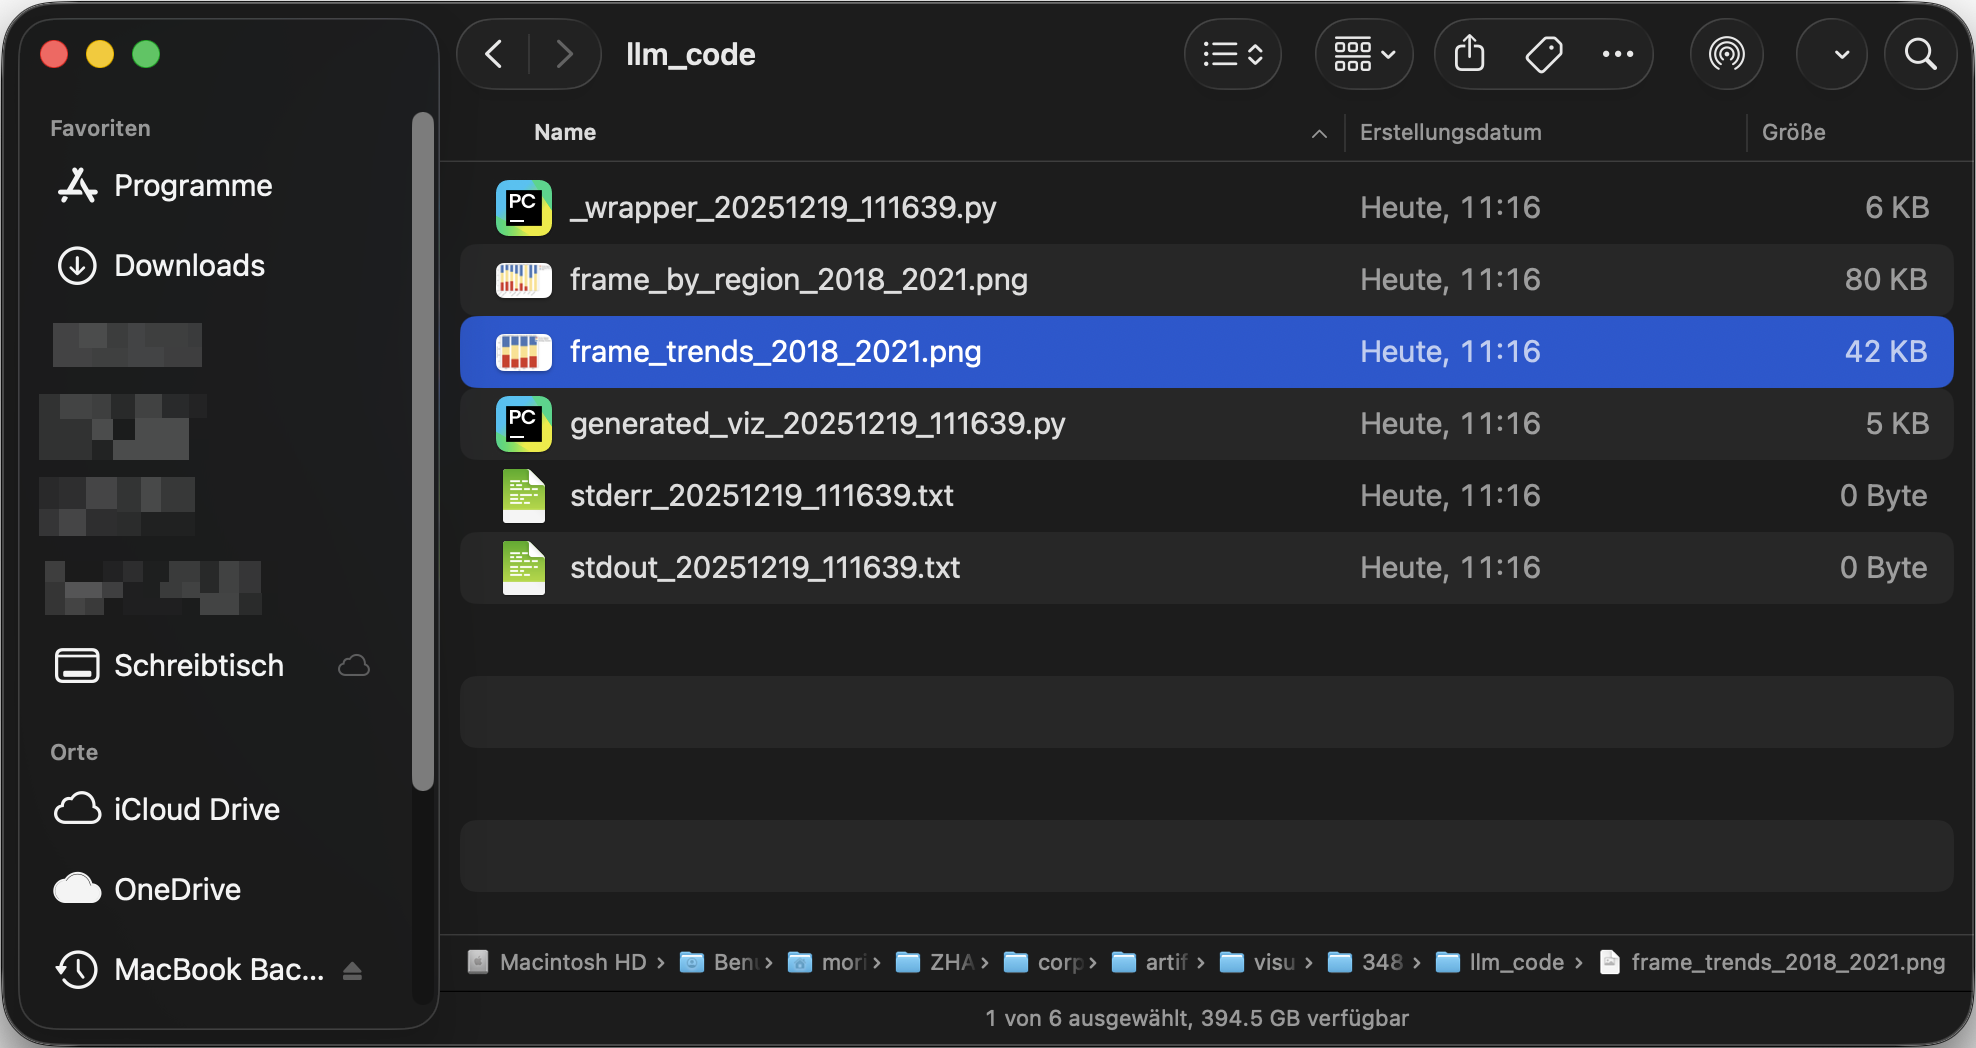
\includegraphics[width=0.95\textwidth]{Figures/walkthrough/ui_09_artifact_folder.png}
    \caption{Visualization artifacts persisted to disk (generated code, wrapper, logs, PNG outputs).}
    \label{fig:ui-artifacts}
\end{figure}

Finally, the visualization pipeline persists all outputs for the run to disk (Figure~\ref{fig:ui-artifacts}). The artifact directory contains the generated plotting script, an execution wrapper, stdout/stderr logs, and the produced PNG files. This persistence supports reproducibility, post-hoc inspection, and iterative refinement of visualization prompts and constraints.


